\section{Closed-loop failure structure}
\label{app:closedloop}

Figure~\ref{fig:closed-loop-behavior} plots the closed-loop behavior summarized in
Table~\ref{tab:closed-loop-behavior} and the final-error contrasts below.

\paragraph{Lower final error does not mean better navigation.}
Weighting reduces mean final navigation error by 0.677 m, with descriptive scene-cluster
interval $[-1.615,+0.010]$. However, it worsens mean closest approach by 0.406 m, interval
$[+0.064,+0.754]$, and changes nDTW by $-0.005$, interval $[-0.031,+0.018]$. Weighted
rollouts leave the agent stationary (executing a turn or a collision-blocked forward, with no position change) on 94.9--96.1\% of steps and visit a median of 1, 2,
and 1 unique positions, versus 18 unweighted. Lower final error and collisions mainly
reflect stationary turns and premature \textsc{stop} actions that replace forward moves, while the closest
approach to the goal gets worse.

\begin{figure}[h]
  \centering
  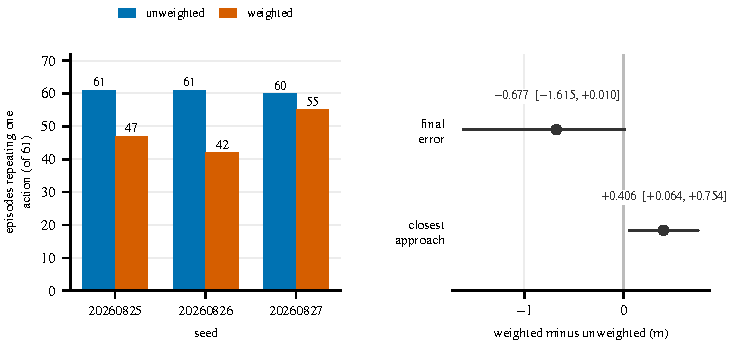
\includegraphics[width=\linewidth]{figures/native_c0_closed_loop_behavior.pdf}
  \caption{\textbf{Closed-loop failure structure.} Left: most weighted episodes repeat one action
  for the full rollout. Right: weighting lowers final navigation error but worsens closest
  approach (positive minimum-distance delta); lines show descriptive $95\%$ intervals from
  resampling the $53$ scenes. SR, OSR, SPL, and SDTW do not improve.}
  \label{fig:closed-loop-behavior}
\end{figure}
